\section{Industry Use Case}
\begin{frame}{}
    \LARGE Object Detection: \textbf{Industry Use Case}
\end{frame}

\begin{frame}[allowframebreaks]{Drainage/Pipeline Internal Defect Detection}
\begin{itemize}
    \item \textbf{Architectures:}
    \begin{itemize}
        \item Improved YOLOv5 (with enhanced CBAM attention, dilated convolution, SIoU loss)
        \item EFE-SSD (with an RFB module for small defects)
        \item Cycle-GAN + YOLOv5 (for data augmentation and detection)
    \end{itemize}

    \item \textbf{Use Case:}
    \begin{itemize}
        \item Underground drainage pipeline defect detection (gravel intrusion, obstacles, foreign objects).
        \item Internal pipeline wall defect detection with image stitching.
        \item Automatic defect detection in CCTV inspection videos.
    \end{itemize}

\framebreak

    \item \textbf{Benefits:}
    \begin{itemize}
        \item Improved YOLOv5 reaches \textbf{64.49\% mAP}, a \textbf{5.27\%} improvement over the YOLOv5 baseline.
        \item EFE-SSD reaches \textbf{92.2\% mAP} across four sewer defect classes, \textbf{2.26 points} above plain SSD.
        \item Cycle-GAN enables \textbf{5.5$\times$} sample augmentation from limited data.
    \end{itemize}

    \item \textbf{Research Papers:}
    \begin{itemize}
        \item \href{https://ascelibrary.org/doi/10.1061/JPSEA2.PSENG-1727}{Zeng et al.\ (Dec 2024)}: enhanced CBAM, switchable atrous and dilated convolution, SIoU loss.
        \item \href{https://www.mdpi.com/2071-1050/15/12/9164}{Shen et al.\ (Jun 2023)}: EFE-SSD, adding an RFB\_s module, ECA attention and focal loss to SSD.
        \item \href{https://pmc.ncbi.nlm.nih.gov/articles/PMC9609589/}{Chen et al.\ (2022)}: Cycle-GAN augmentation, transfer learning from a steel surface-defect dataset, attention mechanism.
    \end{itemize}
\end{itemize}

\framebreak

\begin{figure}
    \centering
    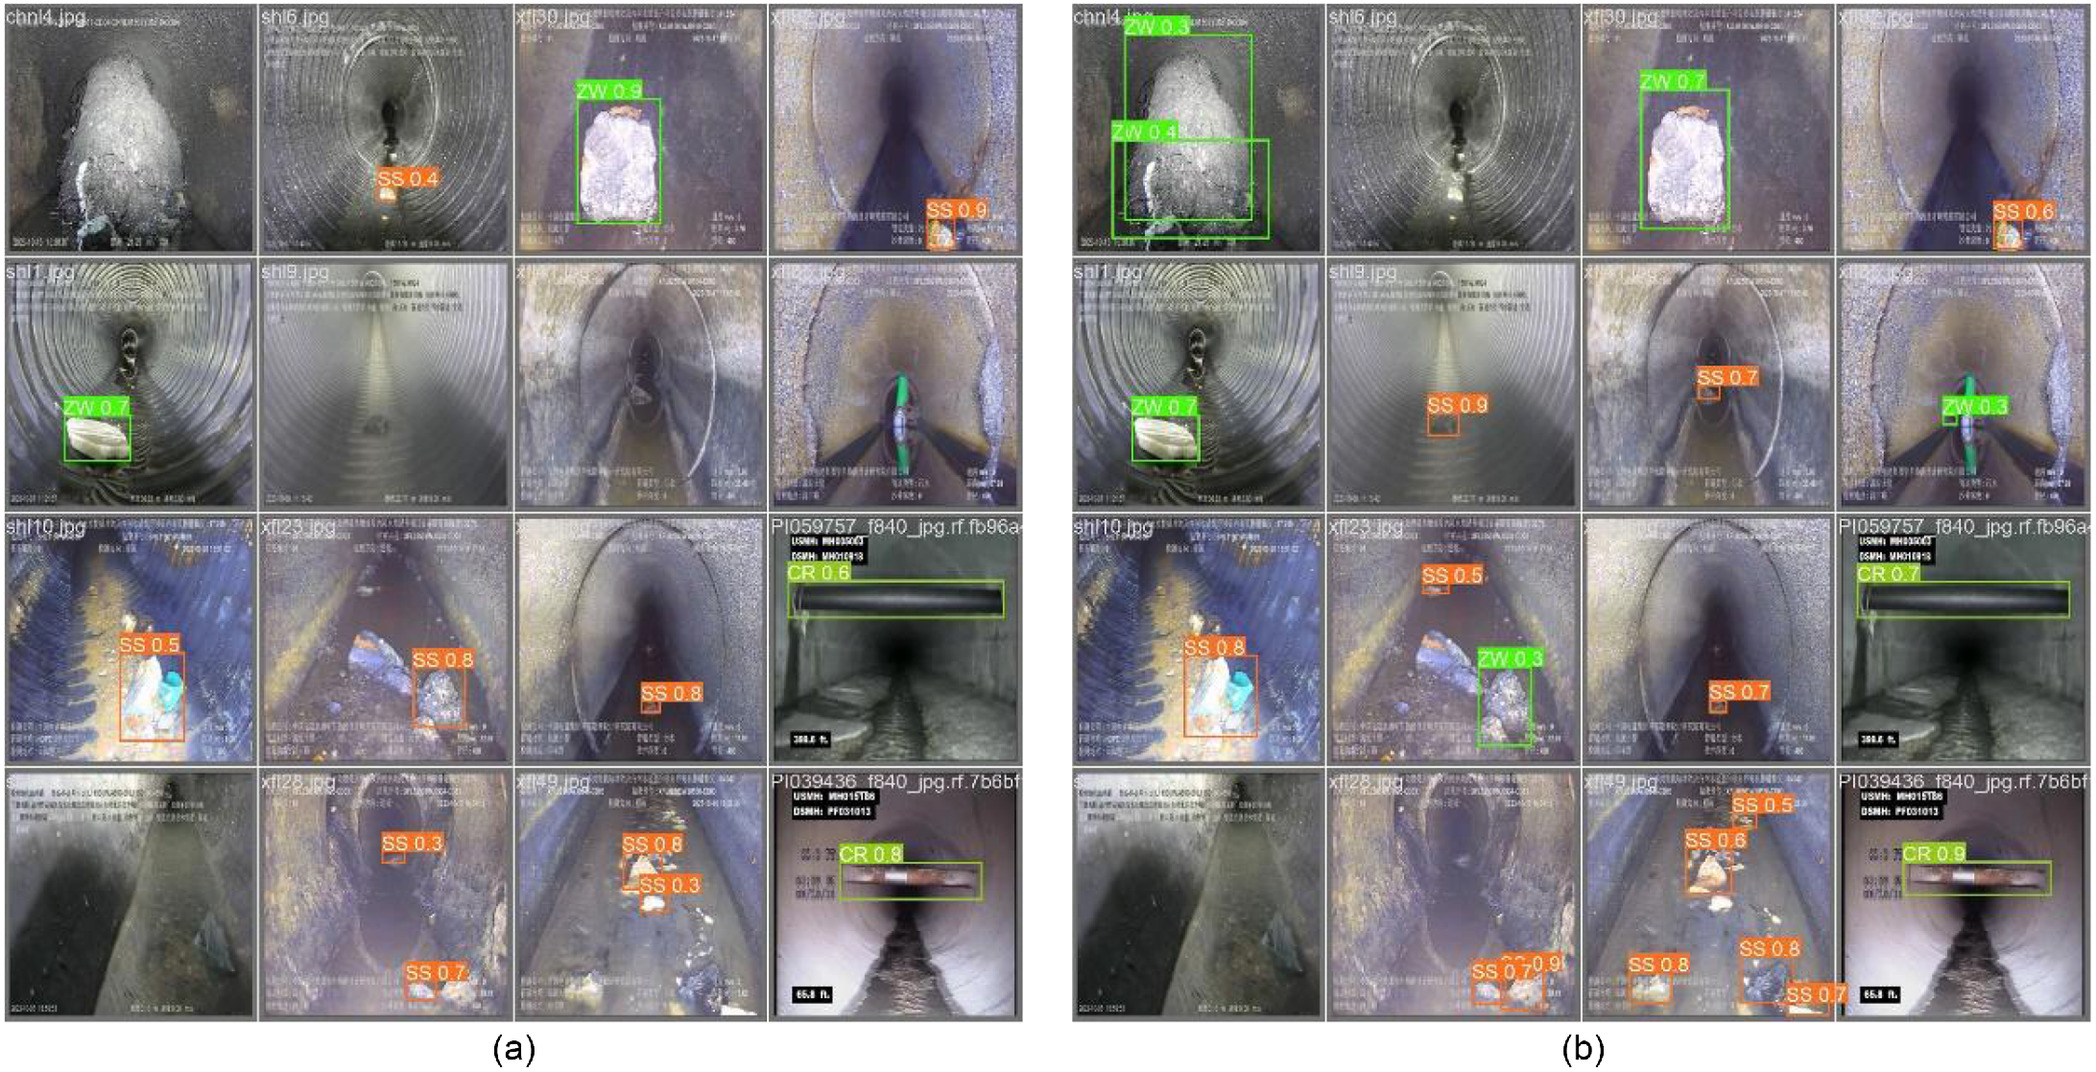
\includegraphics[height=0.75\textheight,width=\textwidth,keepaspectratio]{images/object-detect/yolo5_object_detection.jpg}
    \caption*{\scriptsize The same 16 CCTV inspection frames scored by two detectors, (a) and (b). Each box carries a defect-class code (ZW, SS, CR) and a confidence value; (b) recovers several defects that (a) misses entirely. Source: Zeng et al., ``Research on Improved YOLOv5 Pipeline Defect Detection Algorithm'', \emph{J.\ Pipeline Syst.\ Eng.\ Pract.} 16(2):04024073, 2025, Fig.~9 (CC BY 4.0).}
\end{figure}

\framebreak

\begin{figure}
    \centering
    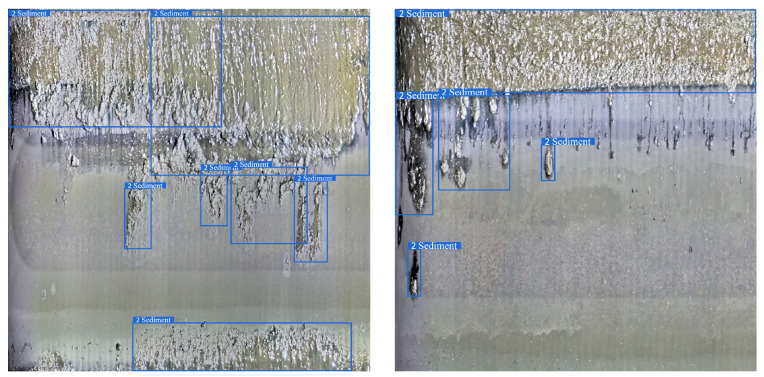
\includegraphics[height=0.7\textheight,width=0.8\linewidth,keepaspectratio]{images/object-detect/sewer_pipe_defect_detection_yolov5.jpg}
    \caption*{\scriptsize YOLOv5 detecting sediment on a stitched drainage-pipe wall. Source: Chen et al., ``An Automatic Defect Detection System for Petrochemical Pipeline Based on Cycle-GAN and YOLO v5'', \emph{Sensors} 22(20):7907, 2022, Fig.~20 (CC BY 4.0).}
\end{figure}
\end{frame}
